\chapter{Testbeams}

\epigraph{I love fools' experiments. \\I am always making them.}{Charles Darwin}

One of the most important aspects of testing and developing DQM4hep was to ensure that it was as generic as it was intended to be, and this meant deploying and using the framework on physics testbeams.

% Sections at the beginning detailing my contributions in the chapter.

[...]

\section{Introduction}

Regular testbeams were held at the DESY II synchrotron at DESY in Hamburg and at the Super Proton Synchrotron (SPS) at CERN. 

[...]

DQM4hep was largely tested and developed during testbeams of the SiWECAL [...]

\section{CALICE testbeams}
[...]

[...] DQM4hep was used in testbeams of the AHCAL over the course of the years 2016-2018, occurring predominantly at the DESY II facility, with one in May 2017 taking place at the CERN SPS.

\subsection{May 2016 at DESY II}
[...] [This was the three-week one, where we got some real shit done.]

Before and during testbeam, the majority of development for AHCAL-specific analysis modules was undertaken. Prior to this, DQM4hep had only been used on SiWECAL beams, and was untested for other detectors. However, file reader and streamer plugins for the SLCIO data format were already present, which meant that the only part needing work was the analysis modules themselves.

To begin with, two analysis modules were developed: 

\begin{itemize}
	\item \texttt{AHCALChannelSpectra} created a histogram for each channel present in the detector, and filled it with the ADC value for each readout cycle in the whole run, producing a per-channel spectrum of ADCs.
	\item \texttt{AHCALHitmap} created a two dimensional histogram, with each bin representing a channel on the $x$ and $y$ axes, and filled each channel with the ADCs of that channel for the whole event, producing a hitmap. 
\end{itemize}

[...]

Creating the hitmap was nontrivial, as the information coming from the data acquisition and stored in SLCIO format did not have geometric information for each channel, instead only specifying the ``electronics number'' -- a combination of the board number and channel number. To determine the location of any given channel, a mapping was needed. This mapping was not simple -- each board contained sixteen channels, and each layer was formed of four boards tiled together. Further, the numbers of the boards and which order the layers were stacked could also change.

For every testbeam, there was a mapping file that described the position of each board and channel in $(i, j, k)$ co-ordinates. To implement the hitmap analysis module, the module used DQM4hep's libraries for XML parsing to build two functions inside the analysis module class --  \texttt{electronicsToIJK} and \texttt{IJKToElectronics} -- that converted either from electronics number to geometric co-ordinates, or vice versa.

Using this method ensured that, given the geometry file was provided, whatever changes in geometry or set-up of the experiment were always reflected in the hitmaps, and no alteration of hard-coded information or recompilation of the modules was required.

[...]

\subsection{December 2016 at DESY II}
[...]

\subsection{May 2017 at CERN SPS}

During May 2017, testbeam time at CERN's Super Proton Synchrotron (SPS) facility was used for further tests for the AHCAL.

\begin{center}
	[Figure: we have plenty of pictures of the testbeam area and the installation.]
\end{center}

[...]

During this testbeam, development of the analysis modules for DQM4hep had largely been completed and the data format of the detector had been fixed for some time. Because of this, after the initial set-up and verification stages, very little management of the monitoring software was necessary. It was instead used as intended -- a tool for shifters to use to troubleshoot problems with the beam or detectors. It was successfully used to identify dead channels on several of the boards [confirm this].

[...]

\begin{center}
	[Plots from the AHCAL CERN testbeam]
\end{center}

\section{DREAM combined testbeam}
[...]

The combined testbeam took place between 5th-12th September 2018 at the CERN SPS beamline facility. [...]

Importantly, none of these detectors or the teams responsible for their construction and operation were part of AIDA-2020, which was useful as a testbed for the generic nature of the DQM4hep framework. Previous testbeams had only used AIDA-2020 detectors, many of which used filetypes or structures defined and standardised within the collaboration, which were already supported by the framework. By attempting to use DQM4hep to monitor non-AIDA-2020, it was possible to test that the design of the framework was truly generic and adaptable to any kind of detector with any filetype.

\subsection{Detectors present at the combined testbeam}
The combined testbeam comprised four separate dectors: a calorimeter, a muon detector and preshower, a drift chamber, and a silicon photomultiplier. One of the biggest challenges involved in the testbeam was operating these four different detectors [...]

\subsubsection{RD52 calorimeter}
The calorimeter was formed of two layers of 36 tiles each, totaling 72 tiles, stacked behind each other. One layer used Cherenkov detectors, the other used scintillator tiles. In addition, there was a group of leakage detectors that detected whether individual events were contained within the calorimeter or not. [DWC - Delayed Wire Chamber?]

\subsubsection{Muon chamber and preshower}
[...]

\subsubsection{Silicon photomultiplier GEM}
[...]

\subsubsection{Drift chamber}
[...]

\subsection{Results}

\subsubsection{File readers}
[...]

The RD52 calorimeter, drift chamber, and muon and preshower were all read using ROOT ntuple files, generated by the DAQ one step after reading and saving the data in a raw binary format. This made the file reader code simpler and more readable, as it simple walked through ROOT trees, extracting data from leaves event-by-event, rather than reading from raw binary or hex information.

For the silicon photomultiplier GEM data, the ``raw'' data format was a text file, containing an XML header followed by a large amount of data in comma-separated values. This file could be loaded directly into DQM4hep, the XML header separated and parsed with DQM4hep's internal XML parsing libraries, and the remaining data parsed. The comma-separated values could be easily parsed using the \texttt{dqm4hep::core::tokenize} function, which takes a string, a delimiter, and a vector, and parses the string into values separated by the delimiter, loading them into the vector. This made extracting the GEM data extremely simple.

\subsubsection{Analysis modules}
[...]

\subsubsection{Data monitoring}
Existing monitoring within the DREAM collaboration could produce accurate histograms from raw data using ROOT, creating plots of the energy spectra of each detector channel per event, along with [other things]. This facility was reproduced in DQM4hep quickly using for-loops in both the C++ code and XML steering files, allowing this to be done with comparatively little code.

Further to this, the flexibility of using C++ code rather than ROOT macros allowed some analysis to be done in a nearly-online fashion. One of the first important quantities is using the RD52 calorimeter data to find $R$ for each event, also called the energy ratio:

\begin{displaymath}
	R = \frac{E_1}{\sum_{i=1}^{10} E_i}
\end{displaymath}

where $E_i$ is the energy of the $i^{th}$ most energetic channel in the event, e.g. $E_4$ is the fourth most energetic channel. Once the ratio $R$ is calculated, a plot can be made of $E_{total}$ vs. $R$ for an entire run that shows separation of electrons from muons and pions -- see Fig. \ref{figure:testbeam/results/EvR}.

\begin{figure}[h]
	\centering
	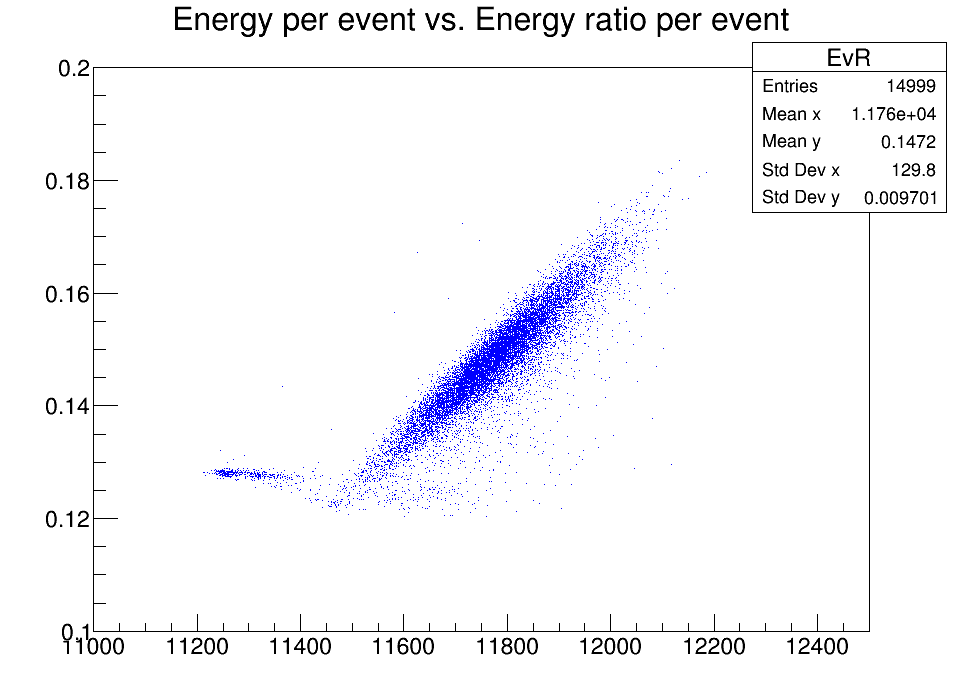
\includegraphics[width=0.65\textwidth]{../Pictures/12709-EvR.png}
	\caption{Plot of $E$ against $R$ for the secondary hadron beam (Run 12709).}
	\label{figure:testbeam/results/EvR}
\end{figure}

An appropriate cut can be used to select electron events. [Information about the cut]. Adding in the information from the RD52's muon trigger, muons and pions can then also be separated. Using both the cut and the muon trigger, we can thus produce spectra for each individual type of particle in the run.

% Although the runs we're talking about here use the secondary hadron beam, so really they should be mostly pions and not much else? I'd say more but information on the beam profile of the SPS is hard to find.

[...]